\chapter{Generative Deep Learning}\label{chp:generative_deep_learning}

\section{Intro to Deep Generative Models}

What Is Generative Modeling?

Generative modeling can be broadly defined as follows:
Generative modeling is a branch of machine learning that involves training a model to produce new data that is similar to a given dataset~\cite{foster2022generative}.

Discriminative models vs Generative models

\paragraph{The Generative Modeling Framework}

\begin{itemize}
	\item We have a dataset of Observations $\mathbf{X}$. \item We assume that the observations have been generated according to some unknown distribution \(\mathcal{P}_{\textrm{data}}\)
	\item We want to build a generative model \(\mathcal{P}_{\textrm{model}}\) that mimics \(\mathcal{P}_{\textrm{data}}\) to generate observations that appear to have been drawn from \(\mathcal{P}_{\textrm{data}}\)
	\item Therefore, the desirable properties of \(\mathcal{P}_{\textrm{data}}\) are:

	      1. Accuracy: if \(\mathcal{P}_{\textrm{model}}\)  is high for a generated observation, it should look like it has been drawn from \(\mathcal{P}_{\textrm{data}}\). If \(\mathcal{P}_{\textrm{model}}\) is low, it should look like it has not been drawn from \(\mathcal{P}_{\textrm{data}}\)

	      2. Generation: it should be possible  to easily sample a new observation from \(\mathcal{P}_{\textrm{model}}\)

	      3. Representation:  it should be possible to understand how different high-level features in the data are represented by \(\mathcal{P}_{\textrm{model}}\)
\end{itemize}

\paragraph{Generative Model Taxonomy}

\begin{itemize}
	\item Explicitly model the density function, but constrain the model in some way, so that the density function s tractable (i.e. it can be calculated)
	\item Explicitly model a tractable approximation of the density function.
	\item Implicitly model the density function, through a stochastic process that directly generates data.
\end{itemize}


\begin{figure}
	\begin{center}
		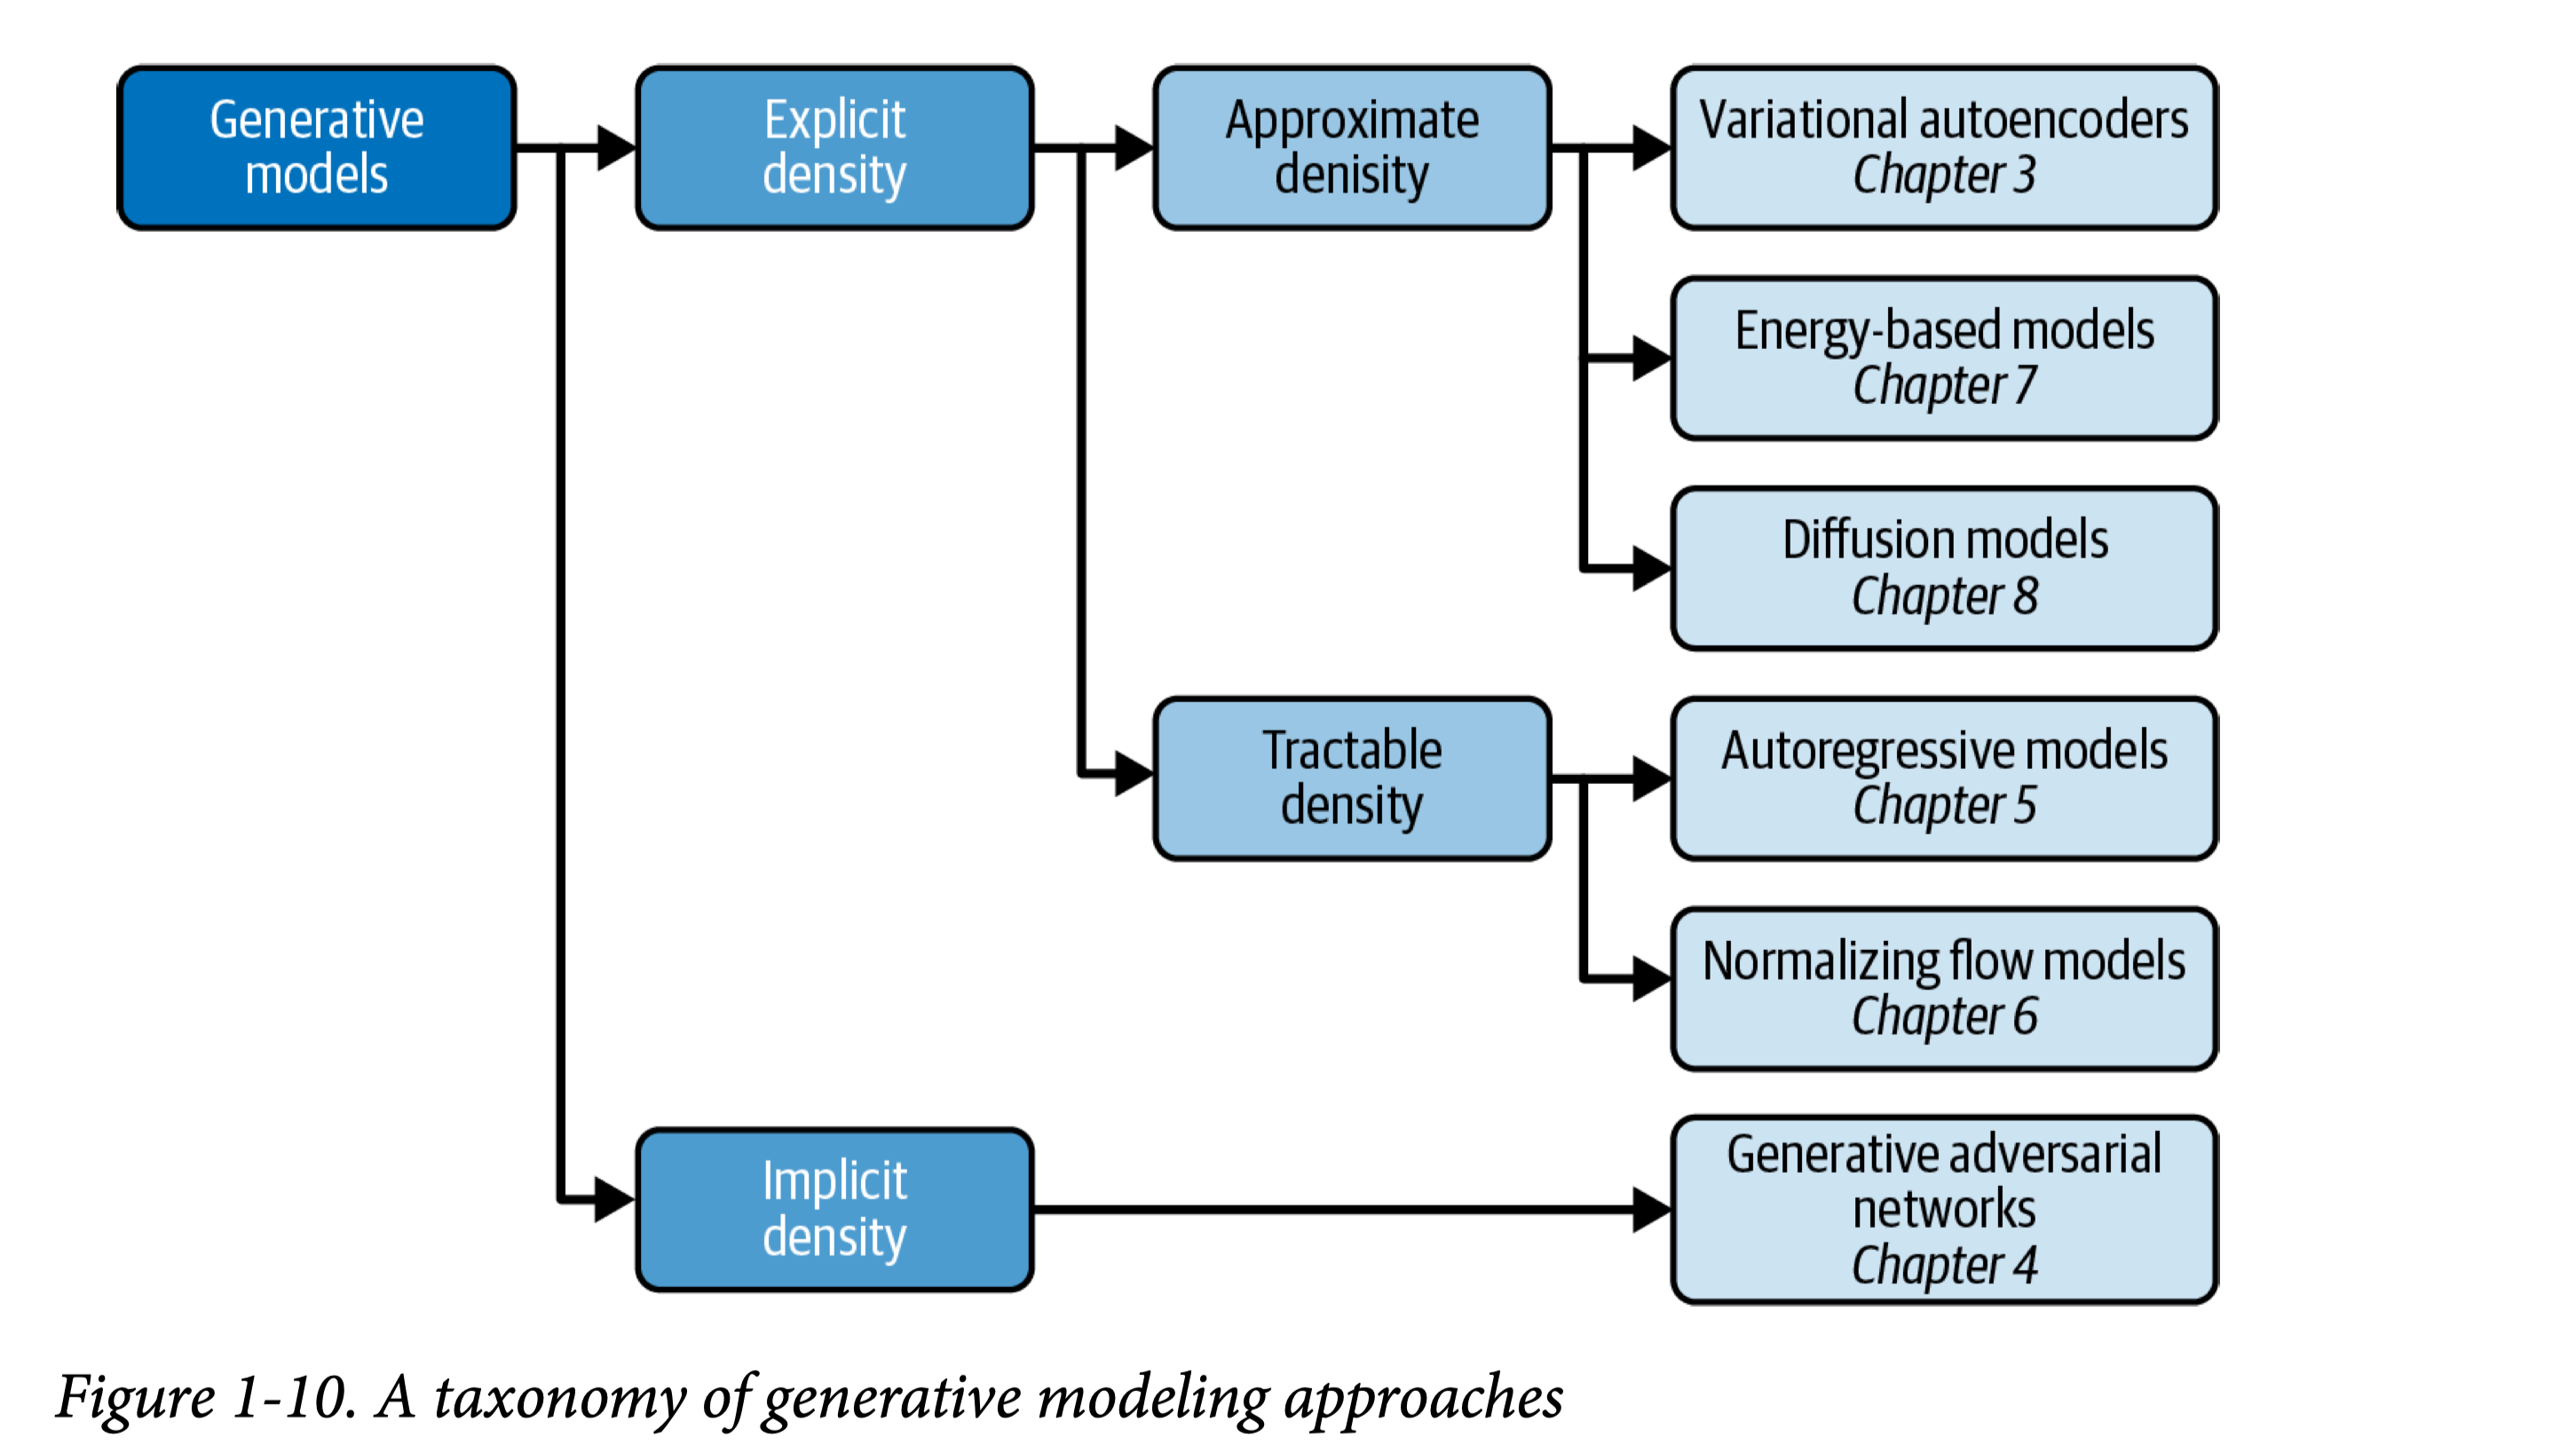
\includegraphics[width=0.95\textwidth]{figures/generative_model_taxonomy}
	\end{center}
	\caption{Generative Models Taxonomy}\label{fig:gmodel_taxonomy}
\end{figure}


If you do choose to use batch normalization before activation, you can remember the order using the acronym \textbf{BAD (batch normalization, activation, then dropout)}


\section{Variational Autoencoders}

\paragraph{The Reparameterization Trick}

Rather than sample directly from a normal distribution with parameters z\_mean and z\_log\_var, we can sample epsilon from a standard normal and then manually adjust the sample to have the correct mean and variance.
This is known as the reparameterization trick, and it’s important as it means gradients can backpropagate freely through the layer.
By keeping all of the randomness of the layer contained within the variable epsilon, the partial derivative of the layer output with respect to its input can be shown to be deterministic (i.e., independent of the random epsilon), which is essential for backpropagation through the layer to be possible.

\paragraph{\gls{kl} Divergence}

\[
	D_{\mathrm{KL}}\left[N\left(\mu,\sigma\right)||N\left(0,1\right)\right] = \frac{1}{2} \sum_{i=1}^n \left(\sigma_i^2 + \mu_i^2 - 1 - \log \sigma_i^2\right)
	.\]


In summary, the \gls{kl}  divergence term penalizes the network for encoding observations to  z\_mean and  z\_log\_var  variables that differ significantly from the parameters of a standard normal distribution, namely \( z\_mean = 0 \) and \( z\_log\_var = 0 \).

Why does this addition to the loss function help?

Firstly, we now have a well-defined distribution that we can use for choosing points in the latent space—the standard normal distribution.
Secondly, since this term tries to force all encoded distributions toward the standard normal distribution, there is less chance that large gaps will form between point clusters.
Instead, the encoder will try to use the space around the origin symmetrically and efficiently.

In the original \gls{vae}  paper, the loss function for a VAE was simply the addition of the reconstruction loss and the KL divergence loss term.
A variant on this (the $\beta$-VAE) includes a factor that weights the \gls{kl}  divergence to ensure that it is well balanced with the reconstruction loss.
If we weight the reconstruction loss too heavily, the \gls{kl} loss will not have the desired regulatory effect and we will see the same problems that we experienced with the plain autoencoder.
If the \gls{kl}  divergence term is weighted too heavily, the \gls{kl}  divergence loss will dominate and the reconstructed images will be poor. This weighting term is one of the parameters to tune when you’re training your VAE~\cite{foster2022generative}.

\paragraph{Latent Space Arithmetic}

One benefit of mapping images into a lower-dimensional latent space is that we can perform arithmetic on vectors in this latent space that has a visual analogue when decoded back into the original image domain~\autoref{fig:vae_latent_space_arithmetic}.

For example, suppose we want to take an image of somebody who looks sad and give them a smile.
To do this we first need to find a vector in the latent space that points in the direction of increasing smile.
Adding this vector to the encoding of the original image in the latent space will give us a new point which, when decoded, should give us a more smiley version of the original image~\cite{foster2022generative}.

\begin{figure}
	\begin{center}
		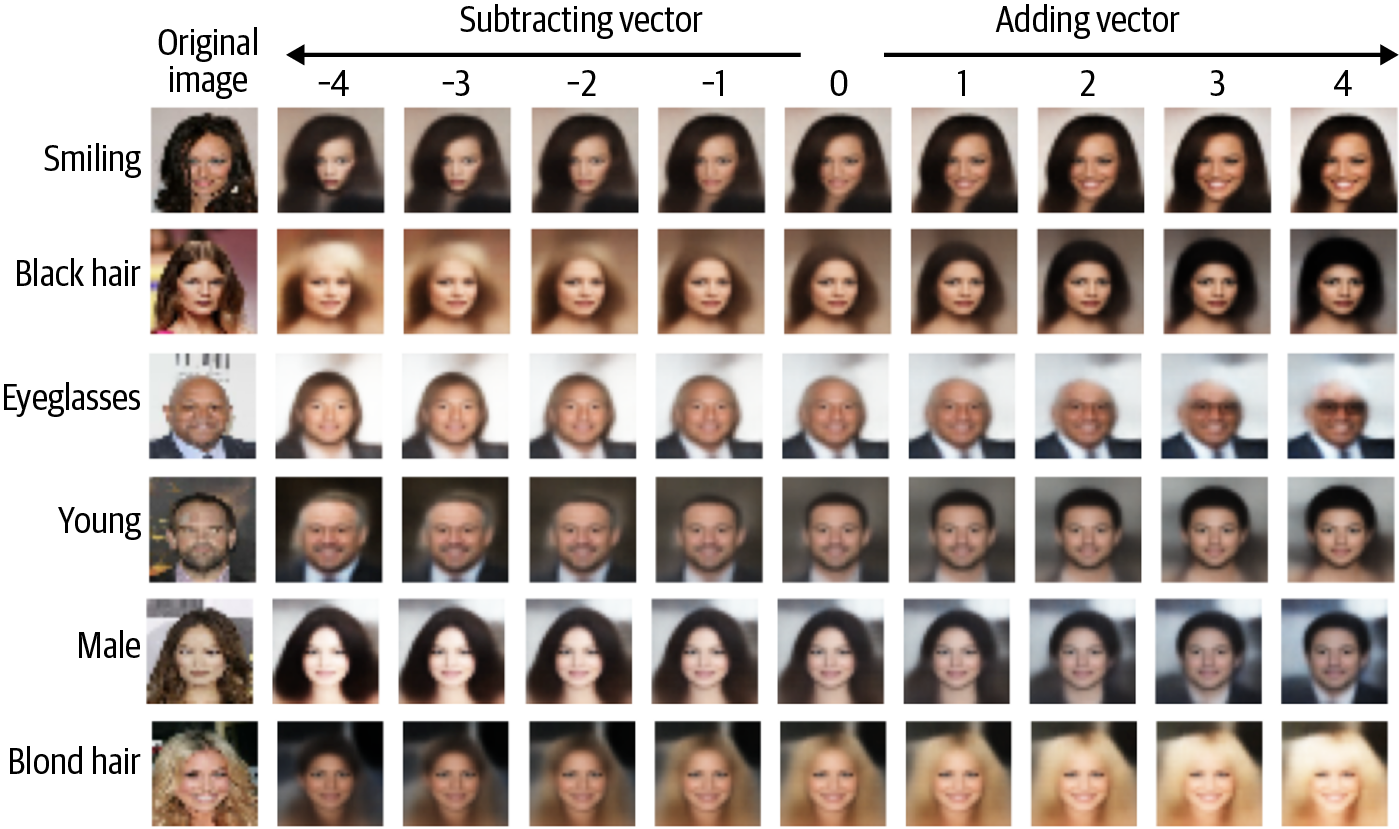
\includegraphics[width=0.95\textwidth]{figures/vae_latent_space_arithmetic}
	\end{center}
	\caption{Adding and subtracting features to and from faces}\label{fig:vae_latent_space_arithmetic}
\end{figure}

\section{Generative Adversarial Networks}

\paragraph{Upsampling vs Transposed Convolution}

The UpSampling2D layer simply repeats each row and column of its input in order to double the size.
The Conv2D layer with stride 1 then performs the convolution operation.
It is a similar idea to convolutional transpose, but instead of filling the gaps between pixels with zeros, upsampling just repeats the existing pixel values.

It has been shown that the Conv2DTranspose method can lead to artifacts, or small checkerboard patterns in the output image (see~\autoref{fig:upsampling}) that spoil the quality of the output.
However, they are still used in many of the most impressive \glspl{gan}  in the literature and have proven to be a powerful tool in the deep learning practitioner’s toolbox.

\begin{figure}
	\begin{center}
		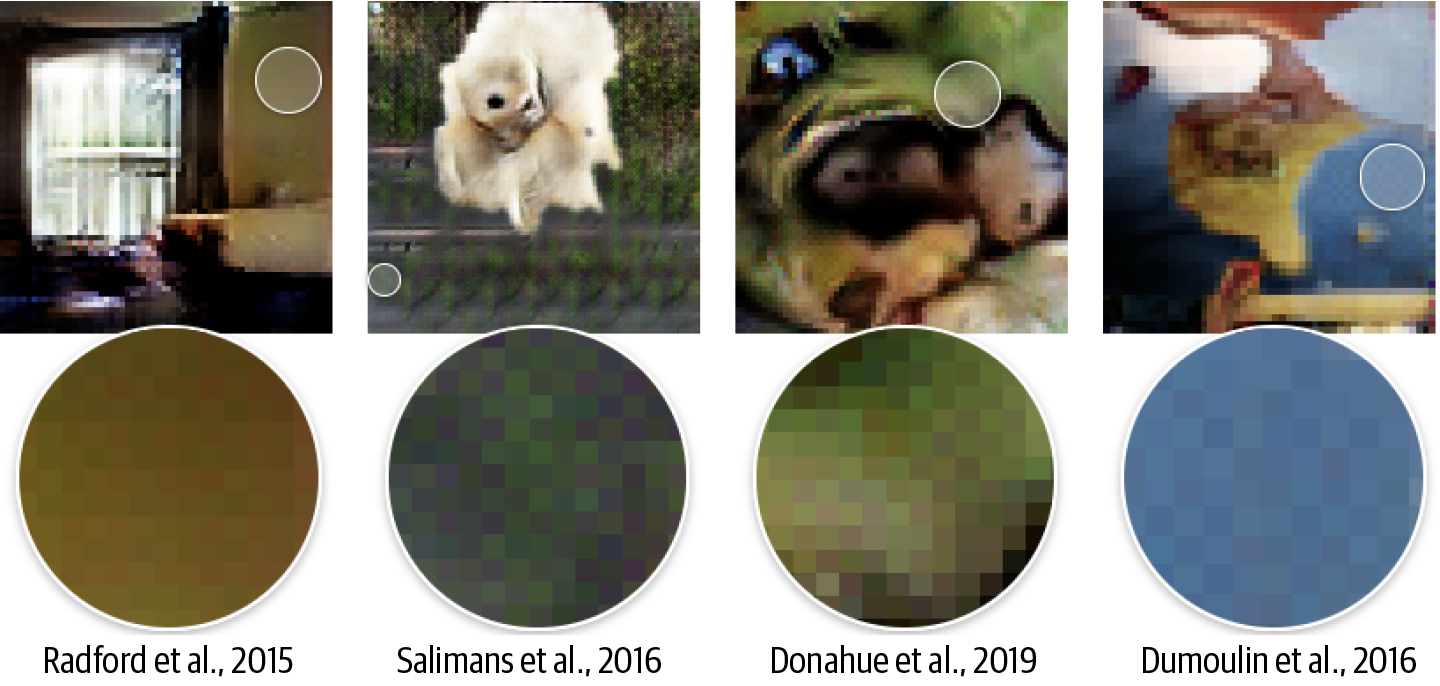
\includegraphics[width=0.9\textwidth]{figures/upsampling}
	\end{center}
	\caption{Artifacts when using convolutional transpose layers}\label{fig:upsampling}
\end{figure}

\paragraph{Adding Noise to the Labels}

A useful trick when training \glspl{gan}  is to add a small amount of random noise to the training labels.
This helps to improve the stability of the training process and sharpen the generated images.
This label smoothing acts as way to tame the discriminator, so that it is presented with a more challenging task and doesn’t overpower the generator.

Another requirement of a successful generative model is that it doesn’t only reproduce images from the training set.
To test this, we can find the image from the training set that is closest to a particular generated example. A good measure for distance is the L1 distance, defined as:

\[
	\mathrm{L1}(\mathbf{a},\mathbf{b}) = \frac{1}{n} \sum_{i=1}^n |a_i - b_i|
	.\]

\subsection{\gls{gan} Training Tips}

While \glspl{gan}  are a major breakthrough for generative modeling, they are also notoriously difficult to train.
We will explore some of the most common problems and challenges encountered when training \glspl{gan}  in this section, alongside potential solutions.
In the next section, we will look at some more fundamental adjustments to the \gls{gan} framework that we can make to remedy many of these problems~\cite{foster2022generative}.

\paragraph{Discriminator overpowering the generator}

If the discriminator becomes too strong, the signal from the loss function becomes too weak to drive any meaningful improvements in the generator.
In the worst-case scenario, the discriminator perfectly learns to separate real images from fake images and the gradients vanish completely, leading to no training whatsoever,

If you find your discriminator loss function collapsing, you need to find ways to weaken the discriminator. Try the following suggestions:

\begin{itemize}
	\item Increase the rate parameter of the Dropout layers in the discriminator to dampen the amount of information that flows through the network.
	\item Reduce the learning rate of the discriminator.
	\item Reduce the number of convolutional filters in the discriminator.
	\item Add noise to the labels when training the discriminator.
	\item Flip the labels of some images at random when training the discriminator.
\end{itemize}

\paragraph{Generator overpowering the discriminator}

If the discriminator is not powerful enough, the generator will find ways to easily trick the discriminator with a small sample of nearly identical images.
This is known as mode collapse.

For example, suppose we were to train the generator over several batches without updating the discriminator in between.
The generator would be inclined to find a single observation (also known as a mode) that always fools the discriminator and would start to map every point in the latent input space to this image.
Moreover, the gradients of the loss function would collapse to near 0, so it wouldn’t be able to recover from this state.

Even if we then tried to retrain the discriminator to stop it being fooled by this one point, the generator would simply find another mode that fools the discriminator, since it has already become numb to its input and therefore has no incentive to diversify its output.

If you find that your generator is suffering from mode collapse, you can try strengthening the discriminator using the opposite suggestions to those listed in the previous section.
Also, you can try reducing the learning rate of both networks and increasing the batch size.

\paragraph{Uninformative Loss}

Since the deep learning model is compiled to minimize the loss function, it would be natural to think that the smaller the loss function of the generator, the better the quality of the images produced.
However, since the generator is only graded against the current discriminator and the discriminator is constantly improving, we cannot compare the loss function evaluated at different points in the training process.
Indeed the loss function of the generator actually increases over time, even though the quality of the images is clearly improving.
This lack of correlation between the generator loss and image quality sometimes makes \gls{gan} training difficult to monitor.

\paragraph{Hyperparameter}

As we have seen, even with simple GANs, there are a large number of hyperparameters to tune.
As well as the overall architecture of both the discriminator and the generator, there are the parameters that govern batch normalization, dropout, learning rate, activation layers, convolutional filters, kernel size, striding, batch size, and latent space size to consider.
GANs are highly sensitive to very slight changes in all of these parameters, and finding a set of parameters that works is often a case of educated trial and error, rather than following an established set of guidelines.

\paragraph{\gls{wgangp}}

\gls{wgangp}~\autoref{fig:wgangp_training} brings a meaningful loss metric that correlates with the generator’s convergence and sample quality, and improved stability of the optimization process.

\begin{figure}
	\begin{center}
		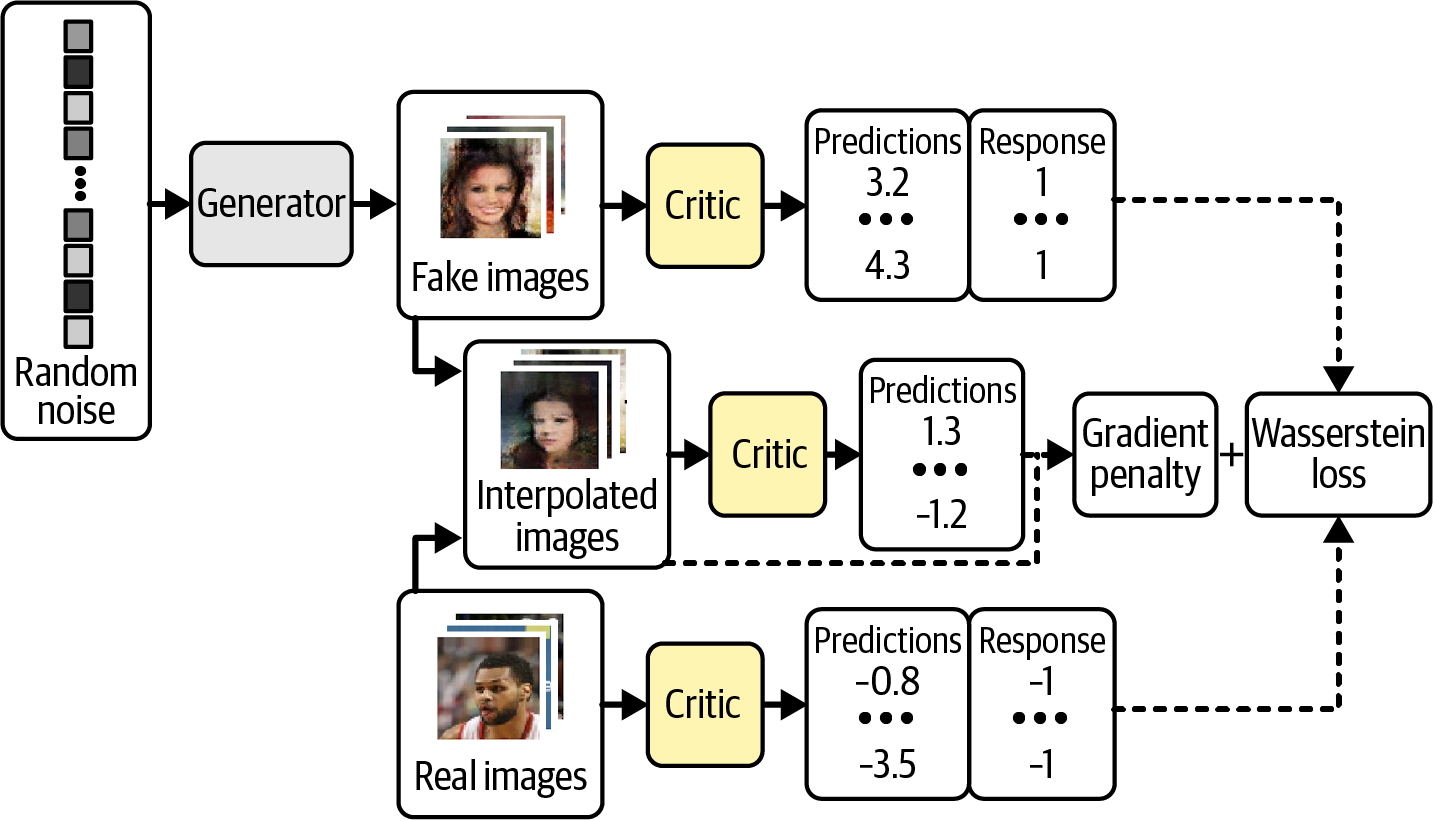
\includegraphics[width=0.95\textwidth]{figures/wgangp_train}
	\end{center}
	\caption{The \gls{wgangp}  critic training process}\label{fig:wgangp_training}
\end{figure}

\begin{equation}
	-\frac{1}{n} \sum_{i=1}^{n} \left(y_i \log\left(p_i\right) + \left(1 - y_i\right)\log \left(1-p_i\right)\right)
	\label{eq:binary_cross_entropy_loss}
\end{equation}

One last consideration we should note before training a \gls{wgangp} is that batch normalization shouldn’t be used in the critic.
This is because batch normalization creates correlation between images in the same batch, which makes the gradient penalty loss less effective.
Experiments have shown that \glspl{wgangp}  can still produce excellent results even without batch normalization in the critic.
We have now covered all of the key differences between a standard GAN and a \gls{wgangp}. To recap:

\begin{itemize}
	\item A \gls{wgangp} uses the Wasserstein loss.
	\item The \gls{wgangp}  is trained using labels of 1 for real and –1 for fake.
	\item There is no sigmoid activation in the final layer of the critic.
	\item Include a gradient penalty term in the loss function for the critic.
	\item Train the critic multiple times for each update of the generator.
	\item There are no batch normalization layers in the critic.
\end{itemize}

\paragraph{\gls{cgan}}

\begin{figure}
	\begin{center}
		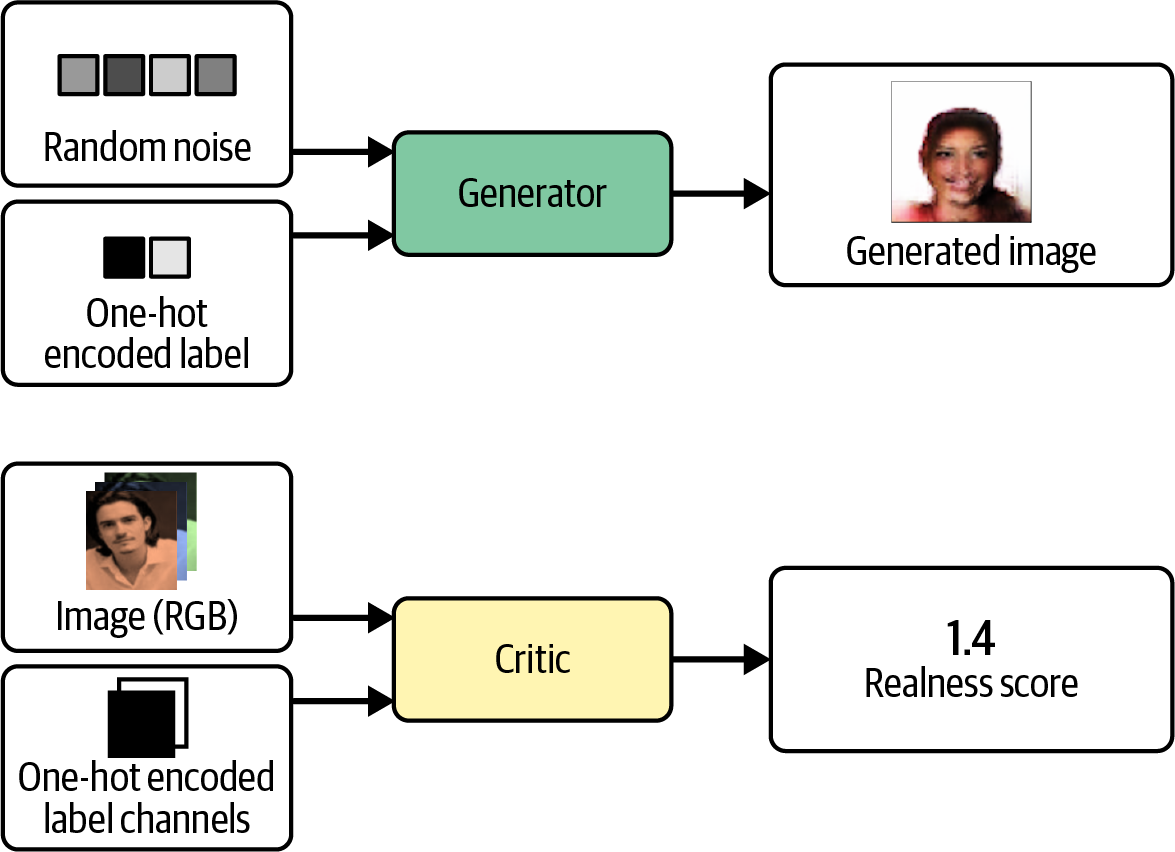
\includegraphics[width=0.95\textwidth]{figures/cgan}
	\end{center}
	\caption{Inputs and outputs of the generator and critic in a CGAN}\label{fig:cgan}
\end{figure}
